 \frame{
 \frametitle{Lukujärjestelmät}
 \begin{itemize}
\item Kymmenjärjestelmä
 \item Binaarijärjestelmä
\item Heksadesimaalijärjestelmä
\item Muunnokset järjestelmästä toiseen
 \end{itemize}
 }

 \frame{
 \frametitle{Kymmenjärjestelmä}
 \begin{itemize}
\item Ihmisten käyttämä numerojärjestelmä on kymmenjärjestelmä eli lukujärjestelmän kantaluku on 10. 
\item Numeromerkkejä on käytössä 10 kappaletta (0--9).
\item Kymmenjärjestelmä on paikkapohjainen eli positiojärjestelmä. Eniten merkitsevä numero on vasemmalla, ja vähiten merkitsevä oikealla.
\item Oikeanpuolimmainen numeromerkki kertoo kantaluvun nollannen potenssin kertoimen, seuraava ensimmäisen potenssin kertoimen ja niin edelleen.
\item Kun halutaan korostaa, mistä lukujärjestelmästä on kysymys, kantaluku merkitään oikeaan alaindeksiin.
 \end{itemize}
\[
123_{10}=1\cdot 10^2 + 2 \cdot 10^1 + 3 \cdot 10^0
\]

 }

 \frame{
 \frametitle{Binaarijärjestelmä eli 2-järjestelmä}
 \begin{itemize}
\item Yleensä käytetään termiä binäärijärjestelmä, koska se sopii suomalaiseen suuhun paremmin. Sanakirjoissa muoto on binaari.\footnote{Ks. esim. Jukka Korpela: Mistä kielestä? (binäärinen vai binaarinen?) http://jkorpela.fi/siv/asu.html }
\item Binaarijärjestelmän kantaluku on 2.
\item 2-järjestelmää käytetään sen yksinkertaisuuden vuoksi digitaali- ja tietotekniikassa.
\item Numeromerkkejä on käytössä kaksi: 0 ja 1.
\[
1111011_2=123_{10}
\]
Muunnos binaarijärjestelmästä kymmenjärjestelmään on helppo: lasketaan vain kahden potenssit yhteen:
\[
1111011_2=1\cdot 2^6+1\cdot 2^5+1\cdot 2^4+1\cdot 2^3+0\cdot 2^2+1\cdot 2^1+1\cdot 2^0= 123_{10}
\] 
\end{itemize}
 }

 \frame{
 \frametitle{Muunnos kymmenjärjestelmästä binaarijärjestelmään}
Jaetaan toistuvasti luvulla 2, ja kirjataan jakojäännös ylös. Esimerkiksi 123 muunnetaan 2-järjestelmään näin:
\begin{eqnarray}
123 &=& 2\cdot 61 +\color{green}1\\
61 &=& 2\cdot 30 +\color{green}1\\
30 &=& 2\cdot 15 + \color{green}0\\
15 &=& 2\cdot 7 + \color{green}1\\
7 &=& 2\cdot 3 +\color{green}1\\
3 &=& 2\cdot 1 +\color{green}1\\
1 &=& 2\cdot 0 +\color{green}1
\end{eqnarray}
\[
123_{10}={\color{green}1111011}_2
\]
 }

 \frame{
 \frametitle{Heksadesimaalijärjestelmä}
 \begin{itemize}
\item Toinen tietokonetekniikassa käytössä oleva lukujärjestelmä on heksadesimaalijärjestelmä. Luvun kantaluku on 16.
\item Kymmenen pienintä numeromerkkiä ovat samat kuin kymmenjärjestelmässäkin. Sitten tulevat merkit A, B, C, D, E ja F.
\item Muunnokset tapahtuvat kuten kymmenjärjestelmästä binaarijärjestelmään (ja päin vastoin) muunnettaessa. Kantalukuna on 16, eli nyt jaetaan kuudellatoista.
 \end{itemize}
\begin{eqnarray}
123 &=& 16\cdot 7 +\color{green}11\\
7 &=& 16\cdot 0 +\color{green}7
\end{eqnarray}
\[
123_{10}={\color{green}7{\rm B}}_{16}
\]

 }

\frame{
 \frametitle{Muunnos binaarijärjestelmästä heksadesimaalijärjestelmään}
Kuusitoista on kahden potenssi, joten muunnos on helppo tehdä ryhmittelemällä. Muunnetaan $1111011_2$ heksadesimaalijärjestelmään:
\[
\underbrace{111}_{7_{10}=7_{16}}\qquad \underbrace{1011}_{11_{10}=\rm B}=7\rm B_{16}
\]

Periaate toimii helposti myös toiseen suuntaan muunnettaessa.
}

 \frame{
 \frametitle{Puolisummain}
\begin{center}
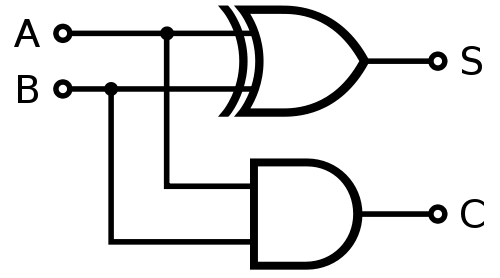
\includegraphics[width=5cm]{lukujarjestelmat_pics/500px-HalfAdder.png} % http://upload.wikimedia.org/wikipedia/commons/thumb/d/d9/Half_Adder.svg/500px-Half_Adder.svg.png
\end{center}


 \begin{itemize}
 \item Tuleva muistibitti (carry in) puuttuu. Soveltuu vain vähiten merkitsevän bitin yhteenlaskuun.
 \end{itemize}
 }

 \frame{
 \frametitle{Kokosummain} % http://upload.wikimedia.org/wikipedia/commons/thumb/a/aa/Full_Adder.svg/500px-Full_Adder.svg.png

\begin{center}
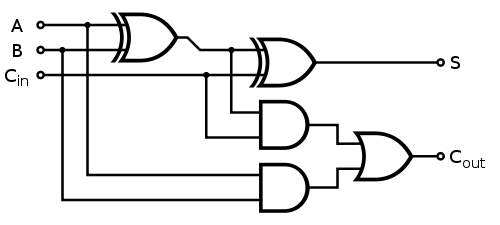
\includegraphics[width=10cm]{lukujarjestelmat_pics/500px-Full_Adder.png}
\end{center}
 \begin{itemize}
 \item Kokosummaimessa on tulo muistibitille, joten niitä voi ketjuttaa monta peräkkäin.
 \end{itemize}
 }


\frame{
 \frametitle{Termistöä}
\begin{description}
\item[bitti] Binaarijärjestelmän numeromerkki, lyhenne b.
\item[tavu] Kahdeksan bitin muodostama yksikkö, lyhenne B.
\item[kibitavu] $2^{10}$ bittiä eli 1024 tavua, lyhenne KiB.
\item[mebitavu] $2^{20}$ bittiä eli 1024 kibitavua eli 1 048 576 tavua, lyhenne MiB.
\end{description}
Bitti on englanniksi bit, tavu on englanniksi byte. Älä sotke niitä keskenään!
Ennen megatavu tarkoitti 1 048 576, mikä oli harhaanjohtavaa, koska kaikkialla muualla tekniikassa mega on $10^6$. Standardiuudistus vuonna 2010 selkiytti termistöä.
}

 \frame{
 \frametitle{Merkistöt}
 \begin{itemize}
 \item Vanhoissa tietokoneissa käytettiin 7-bittisiä merkistöjä, jolloin mahdollisia kirjanmerkkejä oli 128 (ASCII-standardi). 
\item 1990-luvulla siirryttiin 8-bittisiin merkistöihin (esim. ISO 8859-1), jolloin saatiin ääkköset mukaan (256 eri merkkiä). Haittapuolena oli, että eri kielissä on omat erikoismerkkinsä, jolloin tarvittiin useita eri merkistöjä. Jos merkistökoodaus oli valittu väärin, ääkköset näkyivät "pulunkakkoina".\footnote{Legendaarisin esimerkki lienee tahattoman ironinen ilmoitus TKK:n merkistöasiantuntijan potkuista: Jukka Korpelan ty=F6suhde Teknillisess=E4 korkeakoulussa p=E4=E4ttyy.}
\item 2000-luvulla on siirrytty UTF-8-merkistöön, jossa yhtä merkkiä koodataan 1--4 tavulla. Tämä kattaa (käytännössä lähes) kaikki maailman kielten kirjoitusmerkit.
 \end{itemize}
 }
